\section{Design}
This chapter, is dedicated to the high-level design of the presented system. In this chapter we will explain the different concepts used in our policy engine. 

During our brainstorm sessions it quickly became clear that we needed a policy engine that was flexible. With inspiration from other building management systems (see related work) and looking at the web service we had to communicate with, we came up with the concept of policies that consist of rules.

\subsection{Policy}
Merriam-Webster defines policy as; "A definite course or method of action selected from among alternatives and in light of given conditions to guide and determine present and future decisions."

We have defined a policy as a collection of conditional statements operating on sensors and actuators residing in the building simulator. The policy also has a start time and a stop time. It is also possible to de-activate a policy completely - without deleting it entirely.

It's in the statements that the power of our engine lies. A statement can either be a SetStatement or an IfStatement. The Set-statement sets an value in the simulator (in effect it is an actuator). It is possible to have nested If-statements, making the policies both flexible and simple. An If-statement can contain multiple expressions that all are being anded when evaluated. If the user wants to make an If-statement with or between the expressions, she will have to use a nested if. The optimal solution to this would have been to make a safe left-recursive model. We did not have enough time for this, but we will elaborate further on this subject in the discussion (XX REMEMBER THIS XX). An expression can contain the following operators; < > <= >= ! ==. 

For example; lets consider an example where a rooms temperature should be adjusted.

[XX INSERT EXPLANATION XX]

Using this setup allows us to construct rules in a matter similar to other DSL languages such as SQL. Below is an example from a rule we can construct with our engine:
\\
\\
\\
\\
\\
\begin{lstlisting}[language=json,firstnumber=1]
{"statements":[

// Define IF statement
{"type":"IfStatement","data": {"conditionalExpressions":[{"prefixOperator":"AND","aValue":
	{"type":"IntValue","data":{"theValue":10}},"operator":"EQUALS","sensorId":"ROOM1.TEMPERATURE"}],

// Define THEN statement	
	"thenStatements":[{"type":"SetStatement","data":{"aValue":
	{"type":"BooleanValue","data":{"theValue":true}},"sensorID":"ROOM1.HEATER"}}],

// Define ELSE statement
	"elseStatements":[{"type":"SetStatement","data":
	{"aValue":{"type":"BooleanValue","data":{"theValue":true}},"sensorID":"ROOM1.BLINDS"}}]}}]}
\end{lstlisting}

What happens in this example is ...

\subsection{High level design}

\begin{figure}[t]
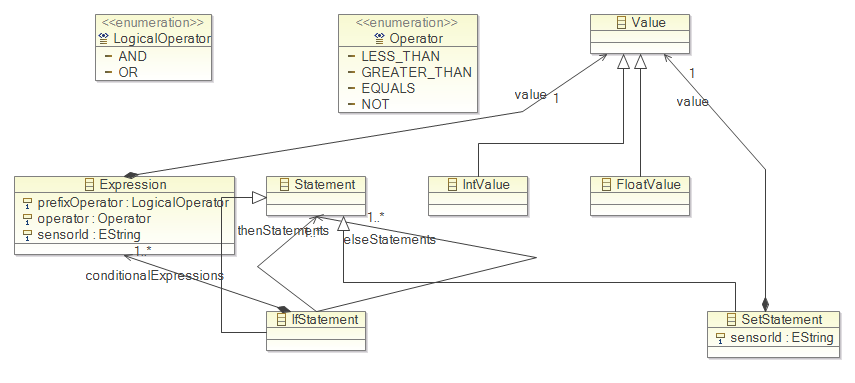
\includegraphics[width=1.00\columnwidth]{model.png}
\caption{Model}
\end{figure}


\subsection{Limitations}
... Alternatives?